\documentclass[submit,techrep,noauthor]{ipsj}

\usepackage{amsmath,amssymb,amsfonts}
\usepackage{cite}
\usepackage[japanese]{babel}
\usepackage[scaled]{beramono}
\usepackage{booktabs}
\usepackage[T1]{fontenc}
\usepackage[dvipdfmx]{graphicx}
\usepackage[utf8]{inputenc}
\usepackage{listings}
\usepackage[all, warning]{onlyamsmath}
\usepackage[subrefformat=parens]{subcaption}
\usepackage{url}

\def\Underline{\setbox0\hbox\bgroup\let\\\endUnderline}
\def\endUnderline{\vphantom{y}\egroup\smash{\underline{\box0}}\\}
\def\|{\verb|}

\begin{document}


\title{ベクトル型スーパーコンピュータ「AOBA-S」の性能評価}

\etitle{Evaluation of a Vector Supercomputer ``AOBA-S''}

\affiliate{CSC}{東北大学サイバーサイエンスセンター}
\affiliate{NEC}{日本電気株式会社}
\affiliate{TU}{東北大学大学院情報科学研究科}
\affiliate{TDU}{東京電機大学}

\author{高橋 慧智,}{Keichi Takahashi}{CSC,TU}[keichi@tohoku.ac.jp]
\author{藤本 壮也,}{Soya Fujimoto}{NEC}[s-fujimoto@nec.com]
\author{長瀬 悟,}{Satoru Nagarase}{NEC}[s.nagase@nec.com]
\author{磯部 洋子,}{Yoko Isobe}{NEC}[y-isobe-pi@nec.com]
\author{下村 陽一,}{Yoichi Shimomura}{CSC,TU}[shimomura32@tohoku.ac.jp]
\author{江川 隆輔,}{Ryusuke Egawa}{TDU}[egawa@mail.dendai.ac.jp]
\author{滝沢 寛之}{Hiroyuki Takizawa}{CSC,TU}[takizawa@tohoku.ac.jp]

\begin{abstract}
東北大学サイバーサイエンスセンターは,2023年8月よりベクトル型スーパーコンピュータ「AOBA-S」の運用を
開始した.AOBA-Sは第3世代ベクトルエンジン (VE30) をノードあたり8基搭載した計504ノードから構成され,
理論演算性能は21.05\,PFLOP/s,メモリ帯域幅は9.97\,PB/sに達する世界最大規模のベクトル型
スーパーコンピュータである.本稿ではAOBA-Sの設計を概説し,運用開始に先駆けて実施したAOBA-Sの
初期性能評価の結果について報告する.
\end{abstract}

%
%\begin{jkeyword}
%情報処理学会論文誌ジャーナル,\LaTeX,スタイルファイル,べからず集
%\end{jkeyword}
%
%\begin{eabstract}
%This document is a guide to prepare a draft for submitting to IPSJ
%Journal, and the final camera-ready manuscript of a paper to appear in
%IPSJ Journal, using {\LaTeX} and special style files.  Since this
%document itself is produced with the style files, it will help you to
%refer its source file which is distributed with the style files.
%\end{eabstract}
%
%\begin{ekeyword}
%IPSJ Journal, \LaTeX, style files, ``Dos and Dont's'' list
%\end{ekeyword}

\maketitle

%1
\section{はじめに}

情報処理学会では,研究報告の発行を行っている.

本稿では,まずそのスタイルファイルを用いた論文のフォーマットに関して述べる.
新たなスタイルファイルでは,
極力特別なコマンドは使わずに,標準的な\LaTeX のスタイルを踏襲している.
論文フォーマットに関しては,\ref{sec:format}~章で後述する指針に従って頂くが,
そこに規定されていること以外は標準的な\LaTeX のコマンドをそのまま使うことができる.
本稿は,そのスタイルファイルを実際に使っているので,論文執筆の際に参考にされたい.


%2
\section{MPI通信性能}

OSU Micro-Benchmarks
7.2\footnote{\url{https://mvapich.cse.ohio-state.edu/benchmarks/}}を用いてMPI通信の性能を計測した.
NCC 5.0.1でコンパイルし,MPIライブラリにNEC MPI 3.4.0を用いた.

\subsection{1対1通信}

図\ref{fig:mpi-lat}に\verb|osu_latency|ベンチマークで計測したMPI 1対1通信のレイテンシを示す.
X.Y節で示した通り,
1.55$\mu$s

\begin{figure}
  \centering
  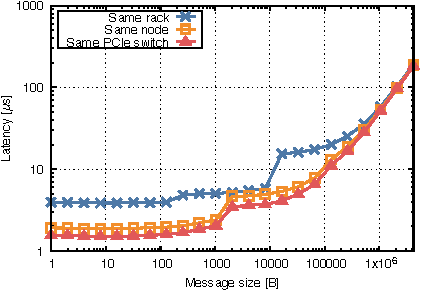
\includegraphics{figs/mpi_latency.pdf}
  \caption{MPI 1対1通信のレイテンシ}\label{fig:mpi-lat}
\end{figure}

\begin{figure}
  \centering
  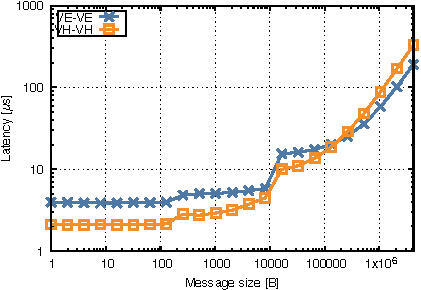
\includegraphics{figs/mpi_latency_vhve.pdf}
  \caption{MPI 1対1通信のレイテンシ}\label{fig:mpi-lat-vh}
\end{figure}

図\ref{fig:mpi-lat}に\verb|osu_bandwidth|ベンチマークで計測したMPI 1対1通信のスループットを示す.

PCIe Gen 4 x16の実効帯域幅31.508\,GB/sである.73.4\%

\begin{figure}
  \centering
  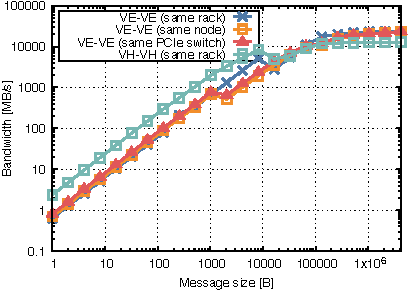
\includegraphics{figs/mpi_bandwidth.pdf}
  \caption{MPI 1対1通信のスループット}\label{fig:bw}
\end{figure}

\begin{figure}
  \centering
  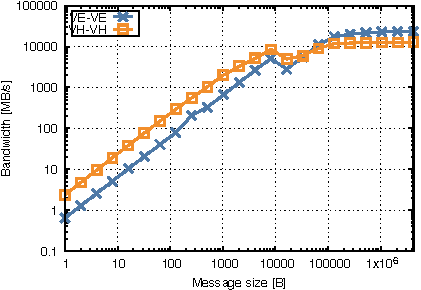
\includegraphics{figs/mpi_bandwidth_vhve.pdf}
  \caption{MPI 1対1通信のスループット}\label{fig:bw-vh}
\end{figure}

\begin{figure}
  \centering
  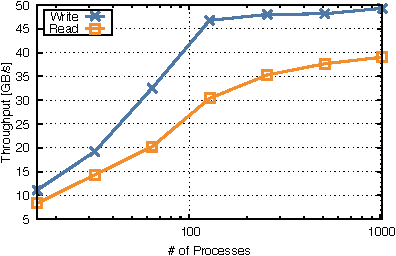
\includegraphics{figs/ior.pdf}
  \caption{並列ファイルシステムのスループット}\label{fig:ior}
\end{figure}

\subsection*{謝辞}

性能評価にご協力いただいた,東北大学情報部デジタルサービス支援課および日本電気株式会社の皆様に
感謝いたします.

\end{document}
